\documentclass{article}

\newenvironment{Itemize}%
{\begin{itemize}%
		\setlength{\itemsep}{0in}%
		\setlength{\topsep}{-.1in}%
		\setlength{\partopsep}{-.1in}%
		\setlength{\parskip}{0in}}%
	{\end{itemize}}

\usepackage{geometry}
\usepackage{amsmath}
\usepackage{mathtools}
\usepackage{amssymb}
\usepackage{epsfig}
\usepackage[TABBOTCAP]{subfigure}
\usepackage{tabularx}
\usepackage{graphicx}
\usepackage{xspace}
\usepackage{thumbpdf}
\usepackage{listings}
\usepackage{verbatim}
\usepackage{hyperref}
\usepackage{booktabs}
\usepackage{colortbl}
\usepackage{hyperref}
\usepackage{color}
\usepackage{xcolor}
\usepackage[utf8]{inputenc}
\usepackage[english]{babel}

\linespread{1.2}

\newtheorem{theorem}{Theorem}[section]
\newtheorem{corollary}{Corollary}[theorem]
\newtheorem{lemma}[theorem]{Lemma}

% To make the FIXMEs go away, comment out this line...
\newcommand{\fixme}[1]{{\bf\textcolor{red}{[#1]}}}
% ...and uncomment this one.
%\newcommand{\fixme}[1]{}
\newcommand{\cut}[1]{}
\newcommand{\xref}[1]{\S\ref{#1}}
\definecolor{darkred}{rgb}{0.7,0,0}
\definecolor{darkgreen}{rgb}{0,0.5,0}
\hypersetup{colorlinks=true,
	linkcolor=darkred,
	citecolor=darkgreen}
\newcommand{\name}{{DeepRM}\xspace}

\newcommand{\hongzi}[1]{{({\color{red}HM: #1})}}
\newcommand{\mohammad}[1]{{({\color{blue}MA: #1})}}
\newcommand{\ishai}[1]{{({\color{green}IM: #1})}}

\hypersetup{pdfstartview=FitH,pdfpagelayout=SinglePage}

\setlength\paperheight {12in}
%\setlength\paperwidth {8.5in}
\setlength{\textheight}{9.25in}
\setlength{\textwidth}{6.8in}
\setlength{\oddsidemargin}{-.1in}
\setlength{\evensidemargin}{-.1in}
%\setlength{\headsep}{0in}
%\pagenumbering{arabic}

\lstset{
	basicstyle=\ttfamily,
	mathescape
}

\lstdefinestyle{customc}{
	belowcaptionskip=1\baselineskip,
	breaklines=true,
	% xleftmargin=20pt,
	language=matlab,
	% frame=L,
	escapeinside={@}{@},
	showstringspaces=false,
	basicstyle=\small\ttfamily,
	keywordstyle=\bfseries\color{green!40!black},
	commentstyle=\itshape\color{purple!40!black},
	%identifierstyle=\color{blue},
	stringstyle=\color{orange},
	% directivestyle=\color{brown},
	%numbers=left,
	%numberstyle=\tiny\color{gray}
}

\lstdefinestyle{customctable}{
	aboveskip=-\medskipamount,
	belowskip=-\medskipamount,
	language=C,
	escapeinside={@}{@},
	showstringspaces=false,
	basicstyle=\scriptsize\ttfamily,
	keywordstyle=\bfseries\color{green!40!black},
	commentstyle=\itshape\color{purple!40!black},
	%identifierstyle=\color{blue},
	stringstyle=\color{orange},
	directivestyle=\color{brown},
}

% Compact itemize and enumerate.  Note that they use the same counters and
% symbols as the usual itemize and enumerate environments.
\def\compactify{\itemsep=0pt \topsep=0pt \partopsep=0pt \parsep=0pt}
\let\latexusecounter=\usecounter
\newenvironment{CompactItemize}
{\def\usecounter{\compactify\latexusecounter}
	\begin{itemize}}
	{\end{itemize}\let\usecounter=\latexusecounter}
\newenvironment{CompactEnumerate}
{\def\usecounter{\compactify\latexusecounter}
	\begin{enumerate}}
	{\end{enumerate}\let\usecounter=\latexusecounter}

\title{Approximation Bounds for Precedence Constrained \\ Job Scheduling Problems}
\author{Hongzi Mao}
\date{December 14, 2016}
\begin{document}
\maketitle

\section{Introduction} \label{s:intro}
Scheduling problems with precedence constraints are among the most difficult
problems in the topic of machine and job scheduling, especially in designing
approximation algorithms. We first present an Integer Linear Program (ILP) for
the general form $P|prec|\sum_j w_jC_j$ of the problem (\S\ref{s:ilp}), which
minimizes the average weighted job completion time on multiple machines under
precedence constraints. Then in \S\ref{s:lpr} we review in details of a
4-approximation algorithm based on LP
relaxation~\cite{queyranne2006approximation}, whose simple form of reading a
list order from LP midpoints actually yields a general framework of precedence
constraints. In the context of single machine scheduling $1|prec|\sum_j w_jC_j$
(\S\ref{s:bism}), interestingly a simple 0-1 bipartite special instance
effectively captures the inherent
difficulty~\cite{woeginger2003approximability}. We review \cite{schulz2011near}
for its new study with a probabilistic lens on the classic 0-1 bipartite
instance, which shows a near optimal solution with large probability in balanced
case. Finally in \S\ref{s:impl}, we implement the ILP and surveyed approximation
algorithms to compare their performance and run time. It verifies the statement
and observations in~\cite{schulz2011near} with a small scale experiment. The
implementations can also be flexibly extended to express the variants of the
problem, such as to also capture the release time constraints, or
multi-dimensional resources constraints.




\section{Problem description} \label{s:problem}
We consider a set $N$ of $n$ jobs, and $m$ identical parallel machines. Each job
$j$ has a nonnegative processing time $p_j$, defined on discrete time stamps $t = 0, 1, 2,
..., T$. Each machine can only be assigned with a single job at a time. We assume no
preemption, meaning each job needs to run continuously once it is assigned to a
machine. The precedence constraints are encoded in a directed acyclic graph
(DAG) $D=(N,E)$: for each precedence-constrained job pair $(i,j) \in E$ job $j$
can not start its execution until job $i$ is finished. Each job $j$ is also associated with a
weight $w_j$. The objective is to minimize the weighted completion time $C_j$
over all jobs $\sum_j w_j C_j$. This general problem is denoted as  $P|prec|\sum_j w_jC_j$
using the notation in~\cite{graham1979optimization}. Also, this model can be tailored to include the makespan objective $P|prec|C_{max}$, which measures the completion time of the last job. We can transform the problem by introducing an artificial job preceded by all other jobs, assigning unit weight and zero processing time to this final job, and leaving all other jobs zero weights. It is well known that the problem is NP-hard, and the major difficulty stems from the precedence constraint, in which even the special case of single machine $1|prec|\sum_j w_jC_j$ is NP-hard \cite{lenstra1978complexity}.
\section{Integer Linear Program} \label{s:ilp}
The general problem of $P|prec|\sum_j w_jC_j$ can be expressed as an optimization problem, which minimizes $\sum_j w_jC_j$, subject to job durations, the precedence constraints and the machine capacity constraints,
\begin{align}
p_j \leq C_j& \:\:\:\: \forall j, \label{eq:ptime}\\
C_i + p_j\leq C_j&  \:\:\:\: \forall (i,j) \in E, \label{eq:prec}\\
\sum_{j | C_j - p_j \leq t \leq C_j} 1 \leq m& \:\:\:\: \forall t \in \mathcal{T}, \label{eq:macap}
\end{align}
where $\mathcal{T}$ is the time horizon of scheduling these jobs and can be upper bounded by $\sum_j p_j$. 

However, the constraint \eqref{eq:macap} is not written in the standard form. To do this, for each job we introduce a time-indexed variable $I_j^t = \{0, 1\}$ to express the constraints. It indicates a single point on the time line at which the job completes its execution, therefore
\begin{align}
\sum_t I_j^t = 1 \:\:\:\: \forall j. 
\end{align}

Notice that $\sum_t tI_j^t = C_j$ captures the time stamp of the job completion event occurring at $t$, and the objective becomes to minimize $\sum_j w_j \sum_t tI_j^t$. We can then translate the precedence constraint \eqref{eq:prec} and capacity constraint \eqref{eq:macap} as 
\begin{align}
\sum_t t I^t_i + p_j \leq \sum_t tI^t_j& \:\:\:\: \forall (i,j) \in E, \label{eq:prec_ti}\\
\sum_{j} \sum_{\tau=t}^{t + p_j} I^\tau_j \leq m& \:\:\:\: \forall t \in \mathcal{T}, \label{eq:macap_ti}
\end{align}
where the second summation in \eqref{eq:macap_ti} effectively acts as a sweeping line to count the overlapping of the job execution at each time stamp over the horizon. 

This framework can be flexibly extended to include other variants of the problem. For instance, jobs may be subject to release time constraint, which can be expressed as $\sum_t tI^t_j \geq s_j + p_j$ to replace \eqref{eq:ptime}, where $s_j$ is the release time of job $j$. Also, each job may also request for multiple types of resources (e.g., CPU and RAM), then the capacity constraints \eqref{eq:macap_ti} can be extended to $\sum_{j} \sum_{\tau=t}^{t + p_j} I^\tau_j r^q_j \leq m^q, \forall q\forall t$, where $q$ indicates each dimension of the resource, $r^q_j$ is the resource requirement of job $j$ and $m^q$ is the capacity of the resource in resource type $q$. In fact, multi-resource precedence constrained job scheduling is suitable for practical datacenter clusters~\cite{graphene}. A production system\footnote{The processing time $p_j$ can actually be estimated in production clusters as a large volume of jobs is consist of recurrent jobs, where the statistics are relatively stable and can be sampled from historical data.} may favor the weighed completion time of the last jobs of each job-group from different applications~\cite{tetris}, which can be included in this framework by assigning $0$ weights to all non-ending jobs.

The main motivation for having this ILP formulation is to implement a baseline to compare against various approximation algorithms in the following sections. 

\section{Approximation Algorithms} \label{s:lpr}

Before a line of classic work of using linear programming (LP) relaxations for designing approximation algorithms of precedence constrained scheduling problems, no constant-factor approximation algorithms were known. In ~\cite{schulz1996scheduling} a 2-approximation algorithms for $1|prec|\sum_j w_jC_j$ is obtained and a 5.3281-approximation algorithms for $P|prec|\sum w_jC_j$ is shown in~\cite{chakrabarti1996improved}. We choose to review the key steps and insights of ~\cite{queyranne2006approximation} in details to show a 4-approximation algorithm for $P|prec|\sum w_jC_j$, since it represents and summarizes this family of algorithms and yields a simple but general framework for the variants of precedence constraints scheduling problems.

The main rounding idea after the LP relaxation is to utilize the solution from LP to construct a priority list of the jobs. Then we can simulate  the time passing forward (to each critical events, e.g., job finished) and schedule the next job in the list, while preserving the capacity constraints and precedence constraints. The construction of such list directly influence the quality of the scheduling. We illustrate in \S\ref{s:lst} and \S\ref{s:lpc}, that a greedy work-conserving job list and the job list from completion time in LP relaxation can lead to very poor result, and actually the midpoint of jobs from LP relaxation leads to the 4-approximation algorithm in \S\ref{s:lpm}.

Unfortunately, the direct LP relaxation of the ILP in \S\ref{s:ilp} is not straightforward to use. If we relax the integer constraint, which captures the job completion time stamp, it breaks the unity of the jobs and thus becomes hard to define the ``mass'' of the jobs for ordering. In order for the LP relaxation to yield a naturally feasible solution, we instead need to use directly the job completion time $C_j$ as the decision variable in \S\ref{s:lprd}, which represents a simplistic way of expressing resource capacity constraints. 

\subsection{List scheduling} \label{s:lst}
LP relaxation for other classic scheduling problem are commonly used with list-scheduling algorithms, which is first introduced in ~\cite{graham1966bounds}. From the solution of the LP relaxation, jobs are sorted based on some rank (e.g., completion time in the solution). Then in the actual scheduling, to satisfy the capacity constraint, whenever a machine becomes available, the next job in the sorted list will be scheduled. To satisfy the precedence constraint\footnote{The job list should not introduce head-of-line blocking, meaning the current head of the job can not be preceded by some job appearing lateral in the list. The feasibility of LP-relaxation solution will prevent this from happening, which will be shown in \S\ref{s:lprd}.}, the next job can only start executing if its predecessors are all finished executing. 

In the presence of precedence constraints, a natural way of assigning job rank is to greedily select the next job if all of its predecessors are already selected. This actually yields a $(2-1/m)$ approximation for the objective of make span ($P|prec|C_{max}$). However, in our weighed completion metric, this can lead to a poor result in the scale of machines counts. 

An example in~\cite{queyranne2006approximation} illustrates this observation: consider $m\geq 3$ machines and three types of jobs, unit-time job $a$, unit-time weight-$1$ jobs $b_1, b_2, ..., b_m$ and m-unit time weight-0 jobs $c_1, c_2, ..., c_{m-1}$. The only precedence constraint is that job $a$ precedes every job in type $b$. The optimal scheduler is to schedule job $a$ first but leave the rest $m-1$ machine idle, so as to schedule type $b$ jobs once $a$ is finished, which leads to its objective value $2m$. The greedy algorithm that keeps resource busy would schedule the jobs of type $c$ in the rest of the machines in the beginning, forcing jobs $b$ being scheduled one after another on the same machine as the job $a$, which results in an objective value $(m+1)(m+2)/2 -1$. Such a greedy list scheduling algorithm is worse than the optimal in the scale of machines $m$ asymptotically.

As the example showed, in some cases we need to deliberately leave an idle time to prevent large-weight jobs, which may become soon in short future, from being blocked by other less important jobs. On the other hand, too much idle time is unnecessary as well. In this sense, LP-relaxation serves as a ``filter" to construct an appropriate job list to balance this tension. 

\subsection{LP-relaxation} \label{s:lprd}
In order to perform LP-relaxation, we now step into another way of expressing the same optimization problem in \S\ref{s:ilp}. The decision variable $C_j$ are kept used as in \eqref{eq:ptime} and \eqref{eq:prec} to capture job duration and the precedence constraints. For machine capacity constraint, we instead write
\begin{align}
\sum_{j\in F} p_j C_j \geq \frac{1}{2m}\left(\sum_{j\in F} p_j \right)^2 + \frac{1}{2}\sum_{j\in F}p_j^2 \:\:\:\: \forall F \subseteq N. \label{eq:mac}
\end{align}
This inequality expresses a convex hull of feasible completion time vectors, which captures the constraint in which each machine can process at most one job at a time. It can be understood in the following derivation. Consider a single machine $i$ and a set of jobs being scheduled in that machine as $F_i$. Without loss of generality, assume the jobs are scheduled are indexed $\{1,2,...,j\} \in F_i$. Since this single machine can only schedule a single job at a time and the job execution is non-preemptive, we have $C_j \geq \sum_{k=1}^j p_k$. Then summing over all jobs in the set, 
\begin{align}
\sum_{j\in F_i} p_j C_j \geq \sum_{j\in F_i} p_j \sum_{k=1}^j p_k = \frac{1}{2} \left[ \left(\sum_{j\in F_i} p_j\right)^2 + \sum_{j\in F_i}p_j^2\right]. \label{eq:ch}
\end{align}

Summing over all machines, the second term becomes directly $\sum_{i=1}^m \sum_{j\in F_i}p_j^2 = \sum_{j\in F}p_j^2$, and the first term has $\sum_{i=1}^m\left(\sum_{j\in F_i} p_j\right)^2 \geq \frac{1}{m}\left(\sum_{j\in F} p_j\right)^2$, due to Cauchy-Schwarz inequality. 

Notice that the relaxation occurs to this linear program when we enforce $F$ to be \emph{any} subset in $N$. Altough there is an exponential number of constraints in \eqref{eq:mac}, \cite{queyranne2006approximation} points out that the separation problem for these inequalities can be solved in polynomial time, thus this LP relaxation can be solved in polynomial time, using ellipsoid method. Because of the scope and the length limit, we refer the proof to \cite{schulz1996scheduling}.

Notice that the solution of the LP relaxation is a feasible solution for the scheduling problem satisfying the precedence and machine capacity constraints. In order for the list-scheduling in \S\ref{s:lst} to present a feasible solution, the ordering of the jobs in the list needs to avoid head-of-line blocking, i.e., the scheduling of the next job in the list is constrained by a job presented lateral in the list. Ordering the job in the list based on any ``location'' of the job $C_j - \alpha p_j$ for any $\alpha \in [0,1]$ would avoid head-of-line blocking. This is because the blocking requires a job $i$ precedes job $j$ and $i$'s finish time is ahead $j$'s starting time. Thus picking a location anywhere in the interval of the job preserves the precedence ordering in the list.

\subsection{Rank on the completion time} \label{s:lpc}
A straightforward way of utilizing LP-relaxation solution is to order the jobs based on their completion time. However, it turns out this can lead to very poor schedules in a meticulously designed example. We consider $m \leq 2$ machines and $m$ sets of jobs $J_h, h\in\{1,2,..,m\}$. Each set $J_h$ contains a long job of processing time $1 + (h-1)(m+1)\epsilon$, $m$ small jobs with processing time $\epsilon$ each. Additionally, there is a final job after all the jobs. The weights of the jobs are all $0$ except for the last job. The precedence constraints are imposed independently on each job set, from the long job to all small jobs. All small jobs then precede the final job. The existence of this final job is to transform the problem from minimizing $\sum_jw_jC_j$ to minimizing makespan $C_{max}$. The construction is illustrated in figure~\ref{fig:lpc}.

\begin{figure}[h]
\centering
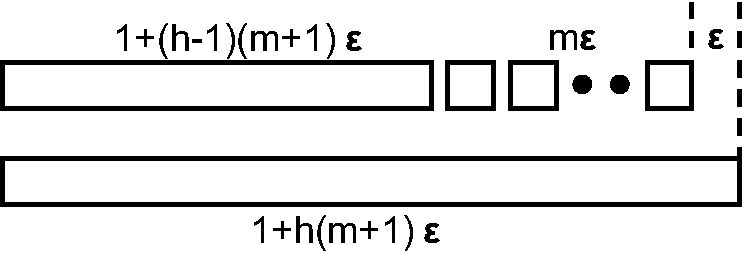
\includegraphics[width=0.5\textwidth]{figs/lpc.pdf}
\caption{List scheduling using the completion time from LP relaxation can lead to poor result in the scale of machines. This example constructs set of small jobs squeezes in front of big jobs as their completion times are earlier.}
\label{fig:lpc}
\end{figure}

The optimal schedule would schedule each long job at the beginning on each machine, then finish all the small jobs in its group immediately one after another. The makespan in this case is effectively the completion time of the last small job of the job set with longest job, which is $(1 + m(m+1)\epsilon) + m\epsilon = 1 +(m^2+2m)\epsilon$. 

Notice that in the optimal solution, each small job in the job set $J_{h-1}$ has completion time earlier than the long job in the next job set $J_h$, as shown in figure~\ref{fig:lpc}. Also, the LP formulation in \S\ref{s:lprd} will find this solution because at the first time step, for the solution to reach the extreme point is to schedule all long jobs (no other jobs can be scheduled because of the precedence constraint), which yields the smallest objective directly. Then putting the priority list with the completion time of the jobs means we put the small jobs of set $J_h$ ahead of the long jobs in the next set $J_{h+1}$. Now scheduling from the list blocks the long job in $J_{h+1}$ being scheduled until all small jobs in $J_h$ finish executing, for every $h$. Therefore, the starting of the long job in $J_h$ is delayed by at least $h$, because it needs to at least wait for all long job in $J_{1, 2,.., h-1}$ to finish. This results in a makespan at least $\sum_h 1 + (h-1)(m+1)\epsilon = m + o(\epsilon)$, which is effectively $m$ times worse than the optimal for sufficiently small $\epsilon$.

\subsection{Rank on the midpoint} \label{s:lpm}
The midpoint is defined as $M_j = C_j - p_j/2$. Instead of sorting the job based on completion time solution in LP relaxation, we use the midpoint from the result. This results in a 4-approximation approximation algorithm for $P|prec|\sum w_jC_j$ as following: Let $C^{LP}$ denotes any feasible solution to the LP relaxation in \S\ref{s:lprd} and $M^{LP}$ denotes the corresponding vector of LP midpoints, let $S_j$ be the vector of start times of the feasible solution constructed by list scheduling using LP midpoints, then

\begin{align}
S_j \leq 4 M^{LP}_j \:\:\:\: \forall j \in N
\end{align}

The proof for this statement is by considering the ``busy hours" and ``free time'' of the machines. Specifically, we denote $\mu$ as the total time before $S_j$ that \emph{all} machines are occupied by some other jobs. This separate the time span before $S_j$ into two kinds of period, busy and idle. We then separately show that the aggregation of all busy period, and idle period are \emph{both} bounded by $2M^{LP}_j$. Namely, we are to show $\mu \leq 2 M^{LP}_j$ and  $S_j - \mu \leq 2 M^{LP}_j$.

The busy period is relatively straightforward. Notice that $\mu$ is upper bounded by $\sum_{i=1}^{j-1} p_i /m$, because the longest consecutive busy hour can be bounded by liquidizing the processing time of all jobs prior to $j$ and assigning them uniformly to all machines. Notice that in \eqref{eq:ch}, if we rearrange the last term in the RHS to the LHS and observe the definition of midpoint $C_j-pj/2 = M_j$, we will have 
\begin{align}
\left(\sum_{i=1}^{j-1}p_i\right)M^{LP}_j \geq \sum_{i=1}^{j-1} p_i M^{LP}_i \geq \frac{1}{2m}\left(\sum_{i=1}^{j-1}p_i\right)^2,
\end{align}
which leads to $\mu \leq \sum_{i=1}^{j-1} p_i /m \leq 2 M^{LP}_j$ as desired. 

\begin{figure}[h]
	\centering
	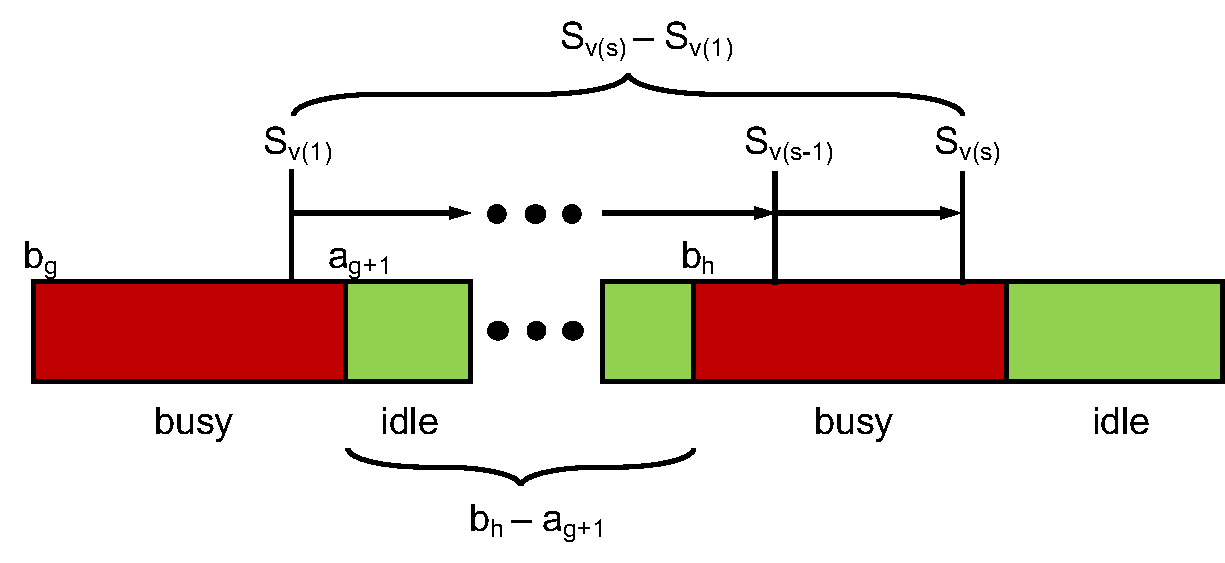
\includegraphics[width=0.6\textwidth]{figs/4-approx-1.pdf}
	\caption{Bound the machine idle period using a set of consecutively scheduled jobs.}
	\label{fig:4-approx}
\end{figure}

On the other hand for the idle period, we aim to show $S_j - \mu \leq 2 M^{LP}_j$, where the LHS is the aggregation of the time period in which at least one machine is idle. The way of reaching this bound is to group the job set that is consecutively running one after another, which in order words saturates the precedence constraints in \eqref{eq:prec}. Specifically, we denote the idle periods as $[a_h, b_h]$. Starting from $S_j$ walking backwards in time, and meet the first busy period we encounter with $b_h$ on its left boundary. We denote $v(1), v(2) .., v(s)$ as the \emph{longest} job span with $v(s)$ has its starting time $S_{v(s)}$ in this encountered busy interval and $S_{v(1)}$ falls out of the busy interval $S_{v(1)} < b_h$. The span of the consecutive jobs is illustrated in figure~\ref{fig:4-approx}. 

First notice that such $v(1)$ exists, because a job starts executing at the boundary $b_h$, and we can at least uses that job as $v(s)$. This job must br preceded on some previous job $v(s-1)$ otherwise it could have been scheduled earlier than $b_h$, since the interval to the left is idle. Secondly, $S_{v(1)}$ has to reside in a busy period $[b_g, a_{g+1})$, because otherwise some machine is idle immediately before the execution of $S_{v(1)}$ and it could have been scheduled earlier. Therefore, as shown in figure~\ref{fig:4-approx}, the span of these consecutive jobs captures some idle periods in the middle. This gives us 
\begin{align}
b_h - a_{g+1} \leq S_{v(s)} - S_{v(1)} = \sum_{i=1}^{s-1}(S_{v(i+1)} - S_{v(1)}) = \sum_{i=1}^{s-1} p_{v(i)}. \label{eq:jobset}
\end{align}

Now we can keep on constructing such consecutive job set spanning the next idle period backward in time, starting inside the busy period of $[b_g, a_{g+1})$ in figure~\ref{fig:4-approx}. The reason is that we can find another starting job time inside the busy period, but has its predecessor starts before $b_g$ (then from the same argument above we know the consecutive job list ends at another busy period), because we can again at least use the job starts at $b_g$ as a new $v(s)$. This way, we can add up all the consecutive time spans to cover all the idle periods. 

Meanwhile, the precedence constraints in \eqref{eq:prec} implies
\begin{align}
M^{LP}_{v(i+1)} \geq M^{LP}_{v(i)} + \frac{1}{2}p_{v(i)} + \frac{1}{2}p_{v(i+1)}. \label{eq:prec2}
\end{align}

Now \eqref{eq:jobset} and \eqref{eq:prec2} can be combined to reach,
\begin{align}
M^{LP}_{v(s)} - M^{LP}_{v(1)} = \sum_{i=1}^{s-1} \left(M^{LP}_{v(i+1)} - M^{LP}_{v(i)}\right) \geq \frac{1}{2}\sum_{i=1}^{s-1} p_{v(i)} \geq \frac{1}{2} (b_h-a_{g+1}),
\end{align}
which now allows us to aggregate all idle periods and to telescope the consecutive job sets to reach $M_j^{LP}$. 

Now combining both busy and idle period, we reach $\mu + (S_j - \mu) \leq 2M_j^{LP} + 2M_j^{LP} = 4M_j^{LP}$, which yields the 4-approximation algorithm.

\section{Probabilistic Analysis} \label{s:bism}
There has been also a line of work focusing primarily on the precedence constraint by studying the single machine case and its special instances. The scheduling problem $1|prec|\sum_jw_jC_j$ is NP-hard and many 2-approximation algorithms exists, such as \cite{hall1997scheduling}. The approximation front already tops the limit since \cite{ambuhl2007inapproximability} showed that PTAS does not exist, assuming NP-complete problems cannot be solved in randomized subexponential time; and \cite{bansal2009optimal} showed that it is even NP-hard to compute a $(2-\epsilon)$ approximated schedule for any $\epsilon> 0$. 

However, from a different angle, the work in \cite{schulz2011near} looks at the problem using a probabilistic lens. It focuses on 0-1 bipartite instances, the simplistic special instance of single machine precedent constrained problem. In bipartite instances, jobs are partitioned into two groups $N_1$ and $N_2$, where the jobs in $N_1$ have unit processing time and zero weight,and the jobs in $N_2$ have zero processing time and unit weight. The precedence constraints are only from group $N_1$ to group $N_2$. In this form, the special instance are  actually completely defined by the precedence constraints.

Even in this simplest scenario, the NP-hardness is actually captured. The difficulty arises really in the dependencies -- multiple jobs in $N_1$ can precede jobs in $N_2$ and the completion of the jobs in $N_2$ will back-propagate to affect the ranks of the parenting jobs. In fact, it turns out these simple instances effectively capture the inherent difficulty of $1|prec|\sum_jw_jC_j$, where ~\cite{woeginger2003approximability} showed that a $\rho$-approximation algorithm for 0-1 bipartite special instances implies a $(\rho+\epsilon)$-approximation algorithm for the general instance of $1|prec|\sum_jw_jC_j$.

Despite this intrinsic hardness, \cite{schulz2011near} interestingly show that for almost all 0-1 bipartite instances, \emph{all feasible schedules are actually arbitrarily close to optimal} with high probability. In other words, they show that for any given $\epsilon > 0$, any feasible schedule is a  $(1 + \epsilon)$-approximation with a large chance, when the number of jobs is sufficiently large. The ``almost-all'' statement assumes the jobs are “balanced” in the 0-1 bipartite instances, in the sense that the ratio between the size of $N_1$ and the size of $N_2$ is not too far from $\Theta(1)$.

The starting point is to use a two-dimensional Gantt charts~\cite{eastman1964bounds} to provide a geometric way of understanding the single-machine completion-time-objective scheduling problems. In figure \ref{fig:gantt}, the horizontal axis corresponds to the processing time, which directly relates to $N_1$ as the jobs of this group has unit processing time and zero weight. Similarly, vertical axis corresponds to the job weights, which relates to job group $N_2$, as they have unit weight and zero processing time. Each job scheduling event (a job in group $N_1$ and the job(s) in group $N_2$ immediately afterwards) represents a ``block'' in the chart, whose horizontal dimension represents the total time (waiting time for the machine and the processing time) of the job in $N_1$ and vertical dimension represents the total weights of the jobs in $N_2$. We plot a work curve using a red line in figure \ref{fig:gantt}, which represents the total weight of jobs that have not been completed by time t. The area under the work curve is equal to the sum of weighted completion times for the schedule represented by the 2D Gantt chart. For example in figure \ref{fig:gantt}, the first job completes at $p_1$ and accounts for $w_1p_1$ of the weighted completion time, where as the second job finishes at $p_1 + p_2$ and results in $w_2(p_1+p_2)$ of the weighted completion time. 
\begin{figure}[h]
	\centering
	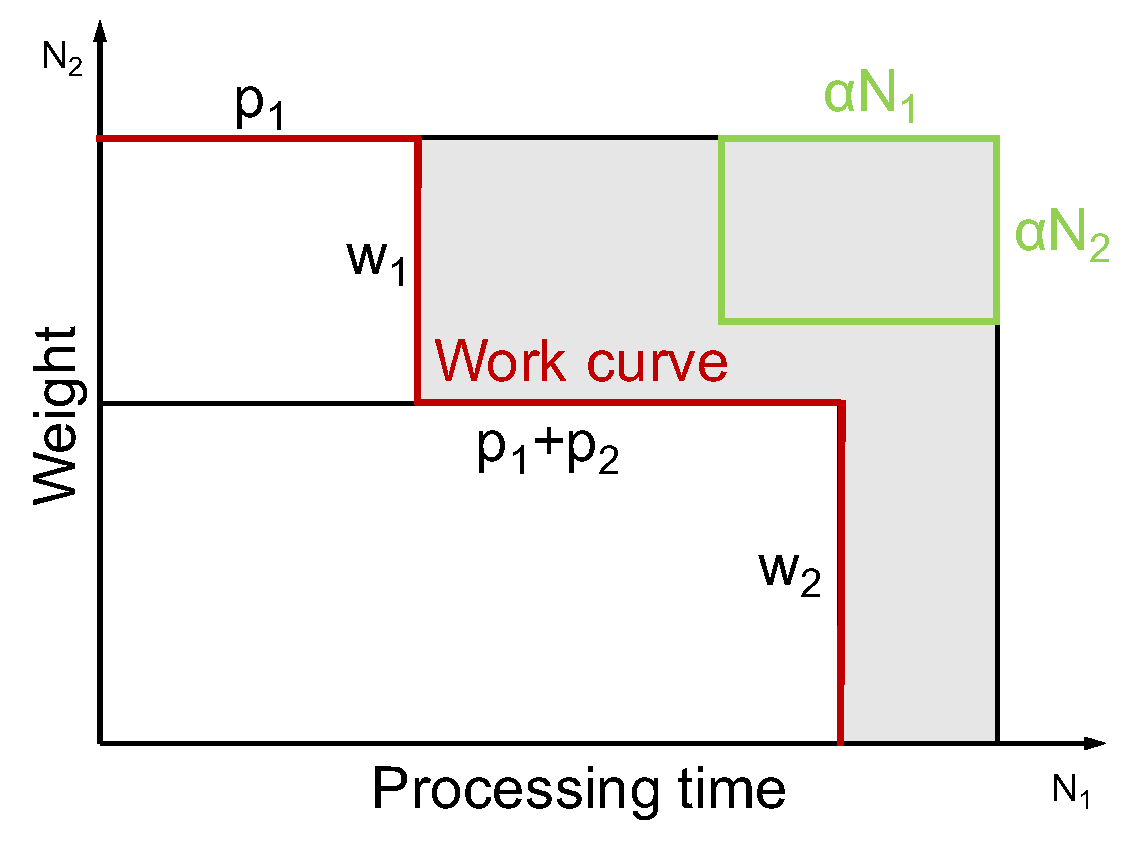
\includegraphics[width=0.5\textwidth]{figs/gantt.pdf}
	\caption{An example of 2D Gantt chart of a 0-1 bipartite instance.}
	\label{fig:gantt}
\end{figure}

The objective is to minimize the sum of total weighted completion time, which effectively is to minimize the area under the work curve. It turns out that the \emph{optimal} work curve has its area under the work curve very large for \emph{almost all} 0-1 bipartite instances. Since the weighted completion time is upper bounded by the total area (where every job finishes at the largest time stamp) of the rectangular Gantt chart, the ``gap" between a feasible solution and the optimal solution is captured by the gray area as shown in figure \ref{fig:gantt}.

We use an ancillary rectangle that is \emph{entirely} contained in the gray area, the green rectangle in figure \ref{fig:gantt}, with a factor $\alpha \in [0,1]$, to quantify the optimality gap. We will show below that the area of this rectangle actually turns out to be arbitrarily small with high probability when the number of machines $n$ is sufficiently large. 

For a desired fixed value $\alpha$, suppose the ancillary rectangle can fit in the gray area, it means there exists a set of $\lceil\alpha n_2\rceil$ jobs from $N_2$ that has at most $n_1 - \lceil\alpha n_1\rceil$ predecessors in $N_1$. In other words, if a rectangle of width $n_1$ and height $n_2$ can fit in the gray area, then there exists a set of $\lceil\alpha n_2\rceil$ jobs from $N_2$ and a set of $\lceil\alpha n_1\rceil$  jobs from $N_1$ with no precedence constraints between them.

Now we show that if the job group $N_1$ and $N_2$ is balanced, and the precedence constrained graph is not extremely sparse, the probability for no constraints between $\lceil\alpha n_1\rceil$ and $\lceil\alpha n_2\rceil$ is small. Suppose the way one can construct a not-so-sparse precedence constraint is that there is a \emph{fixed} probability $q$ for each job in $N_1$ and $N_2$ to establish a precedence dependency. Suppose we are given that the size $|N_1| = s$, and thus $|N_2| = n-s$, then the probability for there to be no precedence constraints between $N_1$ and $N_2$ is bounded by
\begin{align}
{s \choose \lceil\alpha s\rceil}{n-s \choose \lceil\alpha (n-s)\rceil}(1-q)^{ \lceil\alpha s\rceil \lceil\alpha (n-s)\rceil}. \label{eq:constructtwoclass}
\end{align}

Notice that the expoential term over $(1-q)$ decays quickly to $0$ when $n$ is sufficiently large. The rest of the proof in \cite{schulz2011near} is essentially bounding the ${s \choose \lceil\alpha s\rceil}{n-s \choose \lceil\alpha (n-s)\rceil}$ term by forcing the distribution of $s$ to be ``balanced'' with high probability, meaning that the size of $n$ and $n-s$ should be within $\Theta(1)$. The details of the proof is omitted but the insight is that we want to construct the probability distribution $\pi_s$ for $s$, closed to ${n \choose 2} (1/2)^n$, for the size $s=0,1,..,n$. Then notice that ${s \choose \lceil\alpha s\rceil}{n-s \choose \lceil\alpha (n-s)\rceil}$ can be bounded\footnote{Notice that \eqref{eq:constructtwoclass} is conditioned on knowing $s$. To get the completion probability, we need to multiply the distribution of $s$ and sum over them.} by $2^n$ and thus the entire probability can be bounded by $O(n^2 (1-q)^{\alpha^2 s(n-s)})$, which goes to 0 when the number of jobs is sufficiently large. 

Therefore, \cite{schulz2011near} shows that even though the precedence constraint problem is in general difficult, under ``normal'' condition (dependency graph not sparse, job group balanced), an arbitrary feasible solution is actually close to optimal. Notice that the optimality gap here depends on the number of jobs, and this quick expoential decaying property in \eqref{eq:constructtwoclass} hints that the effect should be visible even for the relatively small case for a handful of jobs, which we will test this observation in \S\ref{s:impl}. 
\section{Implementation} \label{s:impl}
We implement the time-indexed based general ILP\footnote{We transform the ILP into its standard form and express the necessary terms as a big matrix, the details are omitted in this report but presented in the actual code.} in \S\ref{s:ilp} and a greedy list scheduling algorithm in \S\ref{s:lst}. The program takes the specification of job weights vector, processing time vector, precedence constraints 0-1 matrix (each $(i, j)$ with entry value 1 indicates $i$ precedes $j$) and number of machines as input, and outputs the weighted sum of completion time, obtained by both ILP and greedy list scheduling. The program can be used for benchmarking approximation algorithms for $P|prec|\sum w_j C_j$ in practice. The code is also open-sourced in \url{https://github.com/hongzimao/6.854/tree/master/project/code}.

We use the implementation to conduct a small scale experiment mainly for the results in \cite{schulz2011near} on the 0-1 bipartite instance. We first did a speed test on ILP approach and the greedy list approach on a 3 parallel machine scenario. The precedence constraints from a direct acyclic graph is randomly generated with the number of constraints uniformly distributed in $[n/2, n]$, where $n$ is the number of jobs. The weights and processing time are uniformly distributed in $[1, 10]$. We then extend to run 100 experiments each on an instance with number of jobs $n = [10, 15, 20, 25, 30]$. Figure \ref{fig:obj_ratio} shows the run time of the two programs averaged over the 100 experiments. As expected, we already see the trend of exponential growing run time in ILP compared with a relatively constant $O(n)$ run time of the list scheduling algorithm.

\begin{figure}[h]
	\centering
	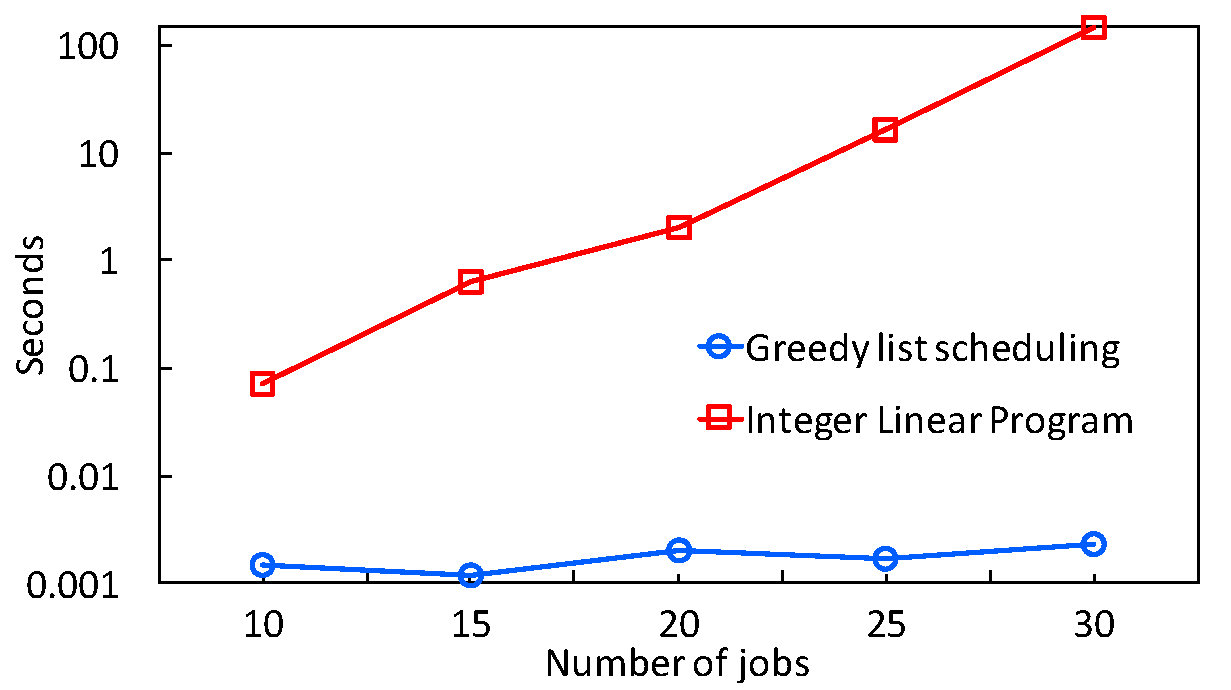
\includegraphics[width=0.6\textwidth]{figs/runtime.pdf}
	\caption{Running time comparison of ILP and simple greedy list scheduling.}
	\label{fig:runtime}
\end{figure}

Then we compare the objective ratio between the list scheduling approximation algorithm and ILP. In a general case of $P|prec|\sum w_j C_j$, as we see in the examples in \S\ref{s:lst} and \S\ref{s:lpc}, we would expect to see the objective ratio between a quickly computed feasible solution and ILP to increase as the number of job grows. In contrast, \S\ref{s:bism} shows the quality of a random solution approaching optimal as the number of job increases. In our experiment for $1|prec|\sum w_j C_j$, we accordingly fix a single machine scenario with 0-1 bipartite types of jobs. Then in 100 experiments with number of jobs $n = [10, 15, 20, 25, 30]$, we randomly assign half of the job to $N_1$ and the other half to $N_2$. For each bipartite pair in $N_1$ and $N_2$, a precedence constrain is established with $0.5$ probability, which satisfies how \S\ref{s:bism} constructs a balanced class. Then we compare the result of the objective ratio in of 3 machine general case and 0-1 bipartite instance in figure \ref{fig:obj_ratio}. The experiment matches with what we expect for the approximation bounds, where the general case has the greedy list scheduling approach progressively worse than optimal as the number of jobs grows, while 0-1 bipartite instance has the phenomenon occurs in the opposite direction. 

\begin{figure}[h]
	\centering
	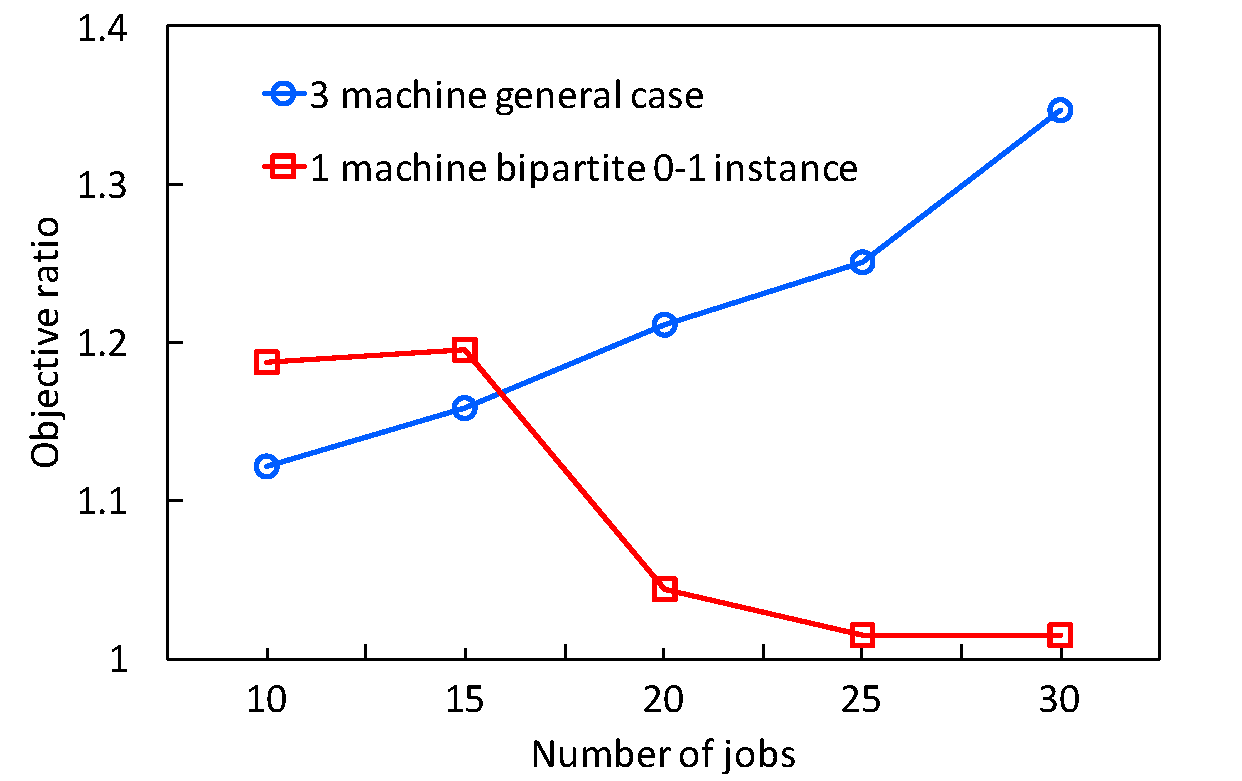
\includegraphics[width=0.6\textwidth]{figs/obj_ratio.pdf}
	\caption{Objective ratio of greedy list scheduling over ILP, on the general 3 parallel machine case and the special bipartite 0-1 instance.}
	\label{fig:obj_ratio}
\end{figure}

\section{Conclusion} \label{s:conclusion}
In this paper, we survey a journey of job scheduling problem with precedence
constraints. In a general form, we presented a time-index based ILP formulation
for the problem in its general case. Then we
follow~\cite{queyranne2006approximation} to construct a 4-approximation
algorithm based on a convex hull LP relaxation, and showed examples where it
outperforms other approaches. For its examples and proof, we clear up the
details and present a simpler description to show the insights and intuitions.
On the other hand, despite the general NP-hardness of the problem even in a 0-1
bipartite instance, we review the fresh study of~\cite{schulz2011near} with a
probabilistic lens to show ``nearly all'' feasible solution is optimal with high
probability, if the number of jobs is sufficiently large. Our implementation on
ILP and a simple greedy list scheduling appraoch for finding feasible solution
show a small scale experiment that matches with the results in this
probabilistic sense. In addition, the code can also be served for further uses
in benchmarking and comparing approximation algorithms. 


\bibliographystyle{alpha}
\bibliography{report}
\end{document}